\section{Experimental Results}

{\color{red} Things to answer.}
\begin{itemize}
\item Are different algorithms affected differently by frequency adjustment?
\item How does frequency affect performance/energy/power?
\item End with SCI cluster and Titan results, and extrapolate from prior 
measurements.
\end{itemize}


\begin{table*}[tb]
  \begin{center}
  %\resizebox{0.95\textwidth}{!}{
  \begin{tabular}{| l | r | r | r | r | r | r | r |}
  \hline
  \textbf{Variant} & \textbf{Performance} & $\mathbf{\frac{Throughput}{Energy}}$ & $\mathbf{\frac{Throughput}{(Energy)^2}}$ & $\mathbf{\frac{(Throughput)^2}{Energy}}$ & $\mathbf{\frac{Throughput}{Power}}$ & $\mathbf{\frac{Throughput}{(Power)^2}}$ & $\mathbf{\frac{(Throughput)^2}{Power}}$ \\ \hline
  \textbf{Merge Sort} & 0 & 0 & 0 & 0 & 0 & 0 & 0 \\ \hline
  \textbf{Radix Sort} & 0 & 0 & 0 & 0 & 0 & 0 & 0 \\ \hline
  \end{tabular}
  %}
  \end{center}
  \caption{Distribution of variant selections across inputs}
  \label{tab:ss}
\end{table*}

\begin{figure*}[tb]
   \centering
   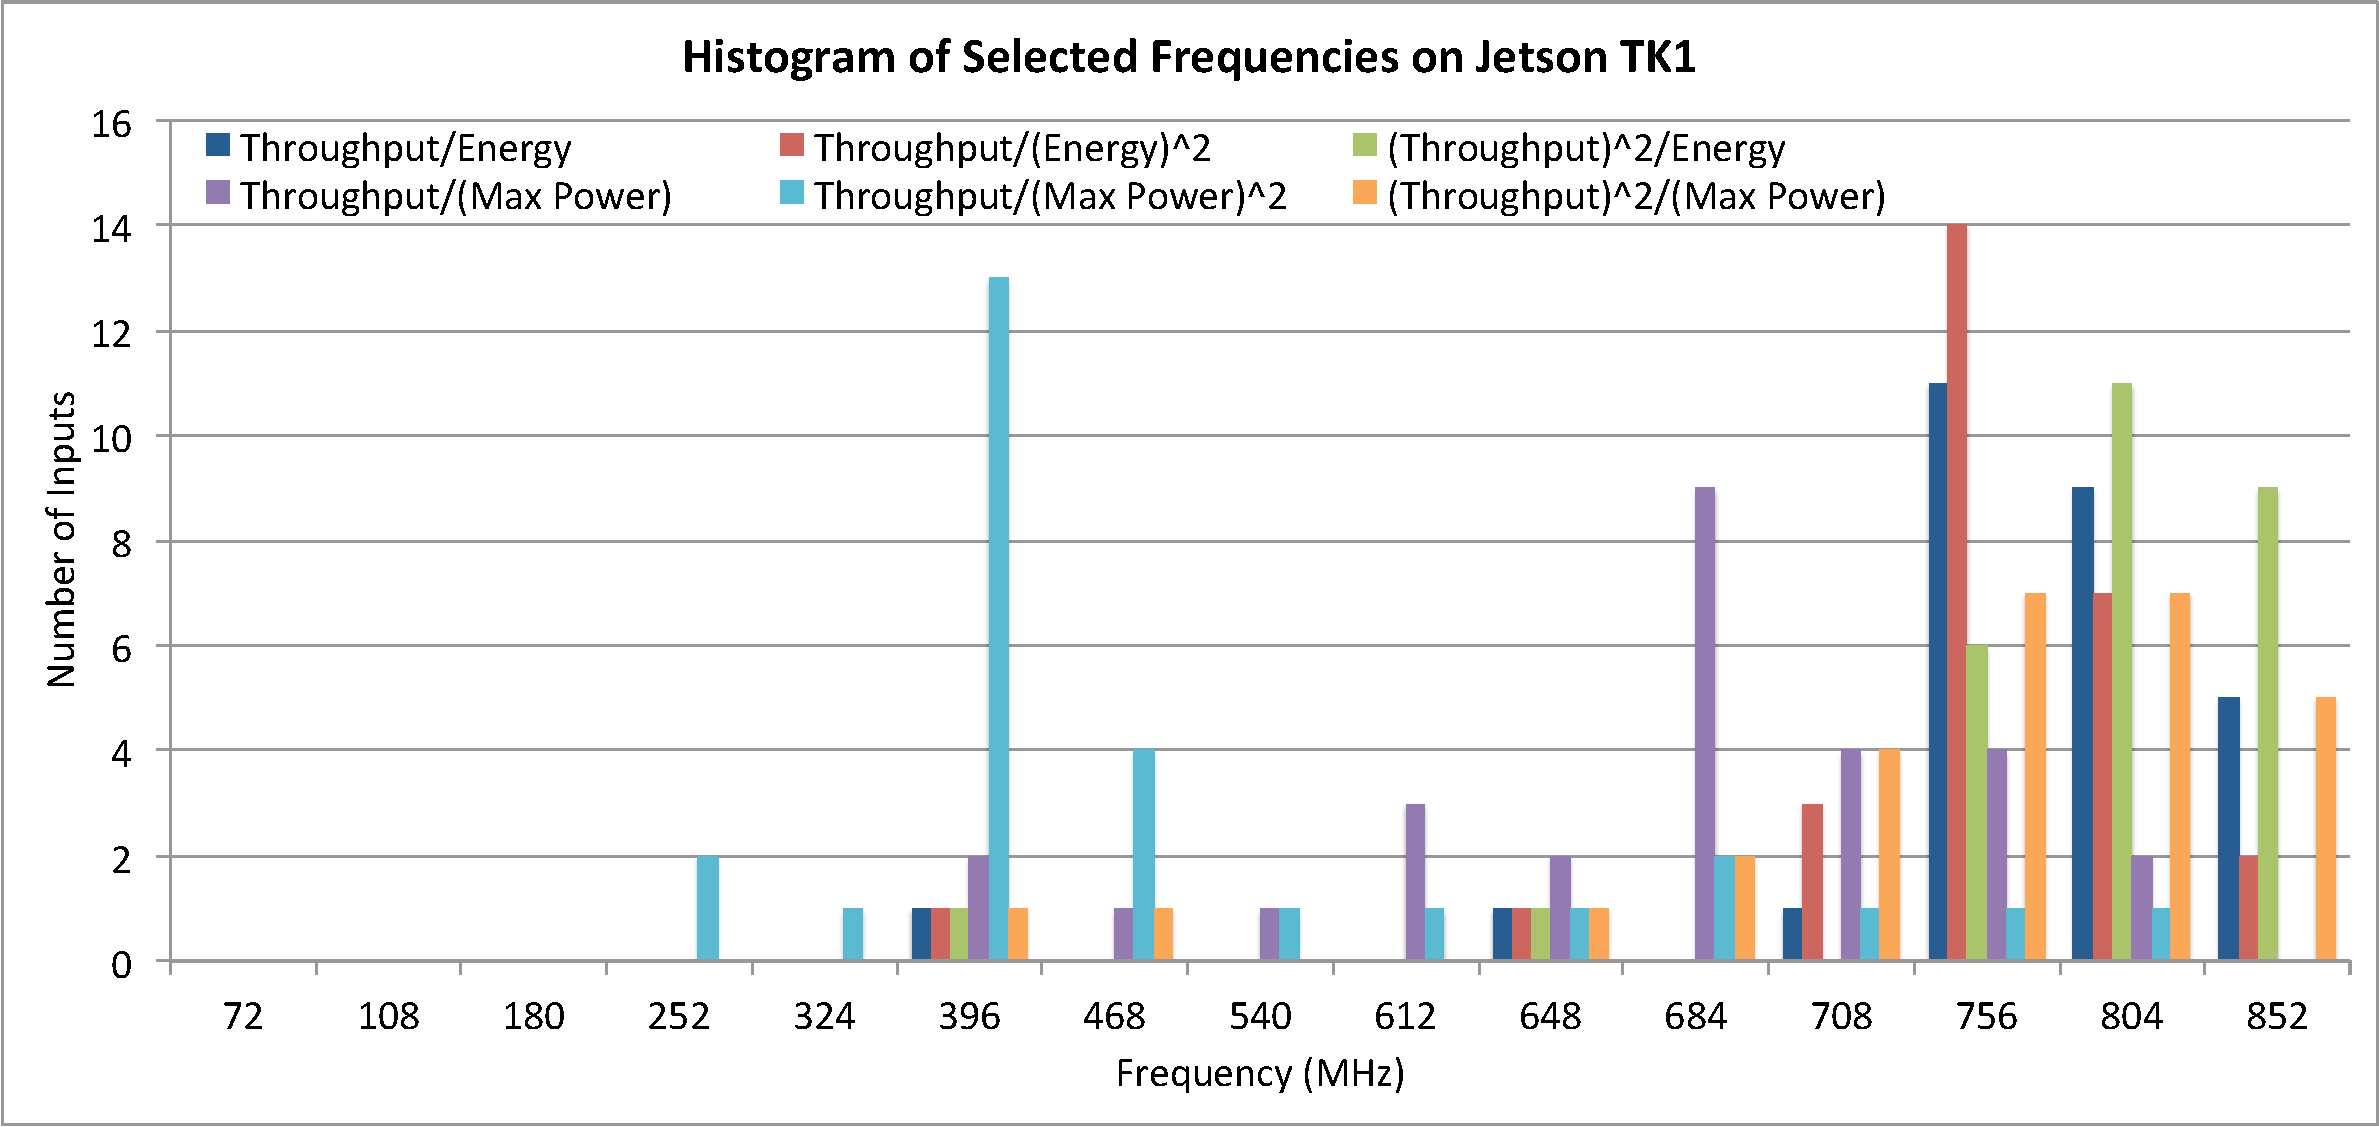
\includegraphics[scale=0.4]{figs/histo_tk1.pdf}
   \caption{Frequencies selected on the Jetson TK1 for various optimization objectives}
   \label{fig:histo-tk1}
\end{figure*}

\begin{figure*}[tb]
   \centering
   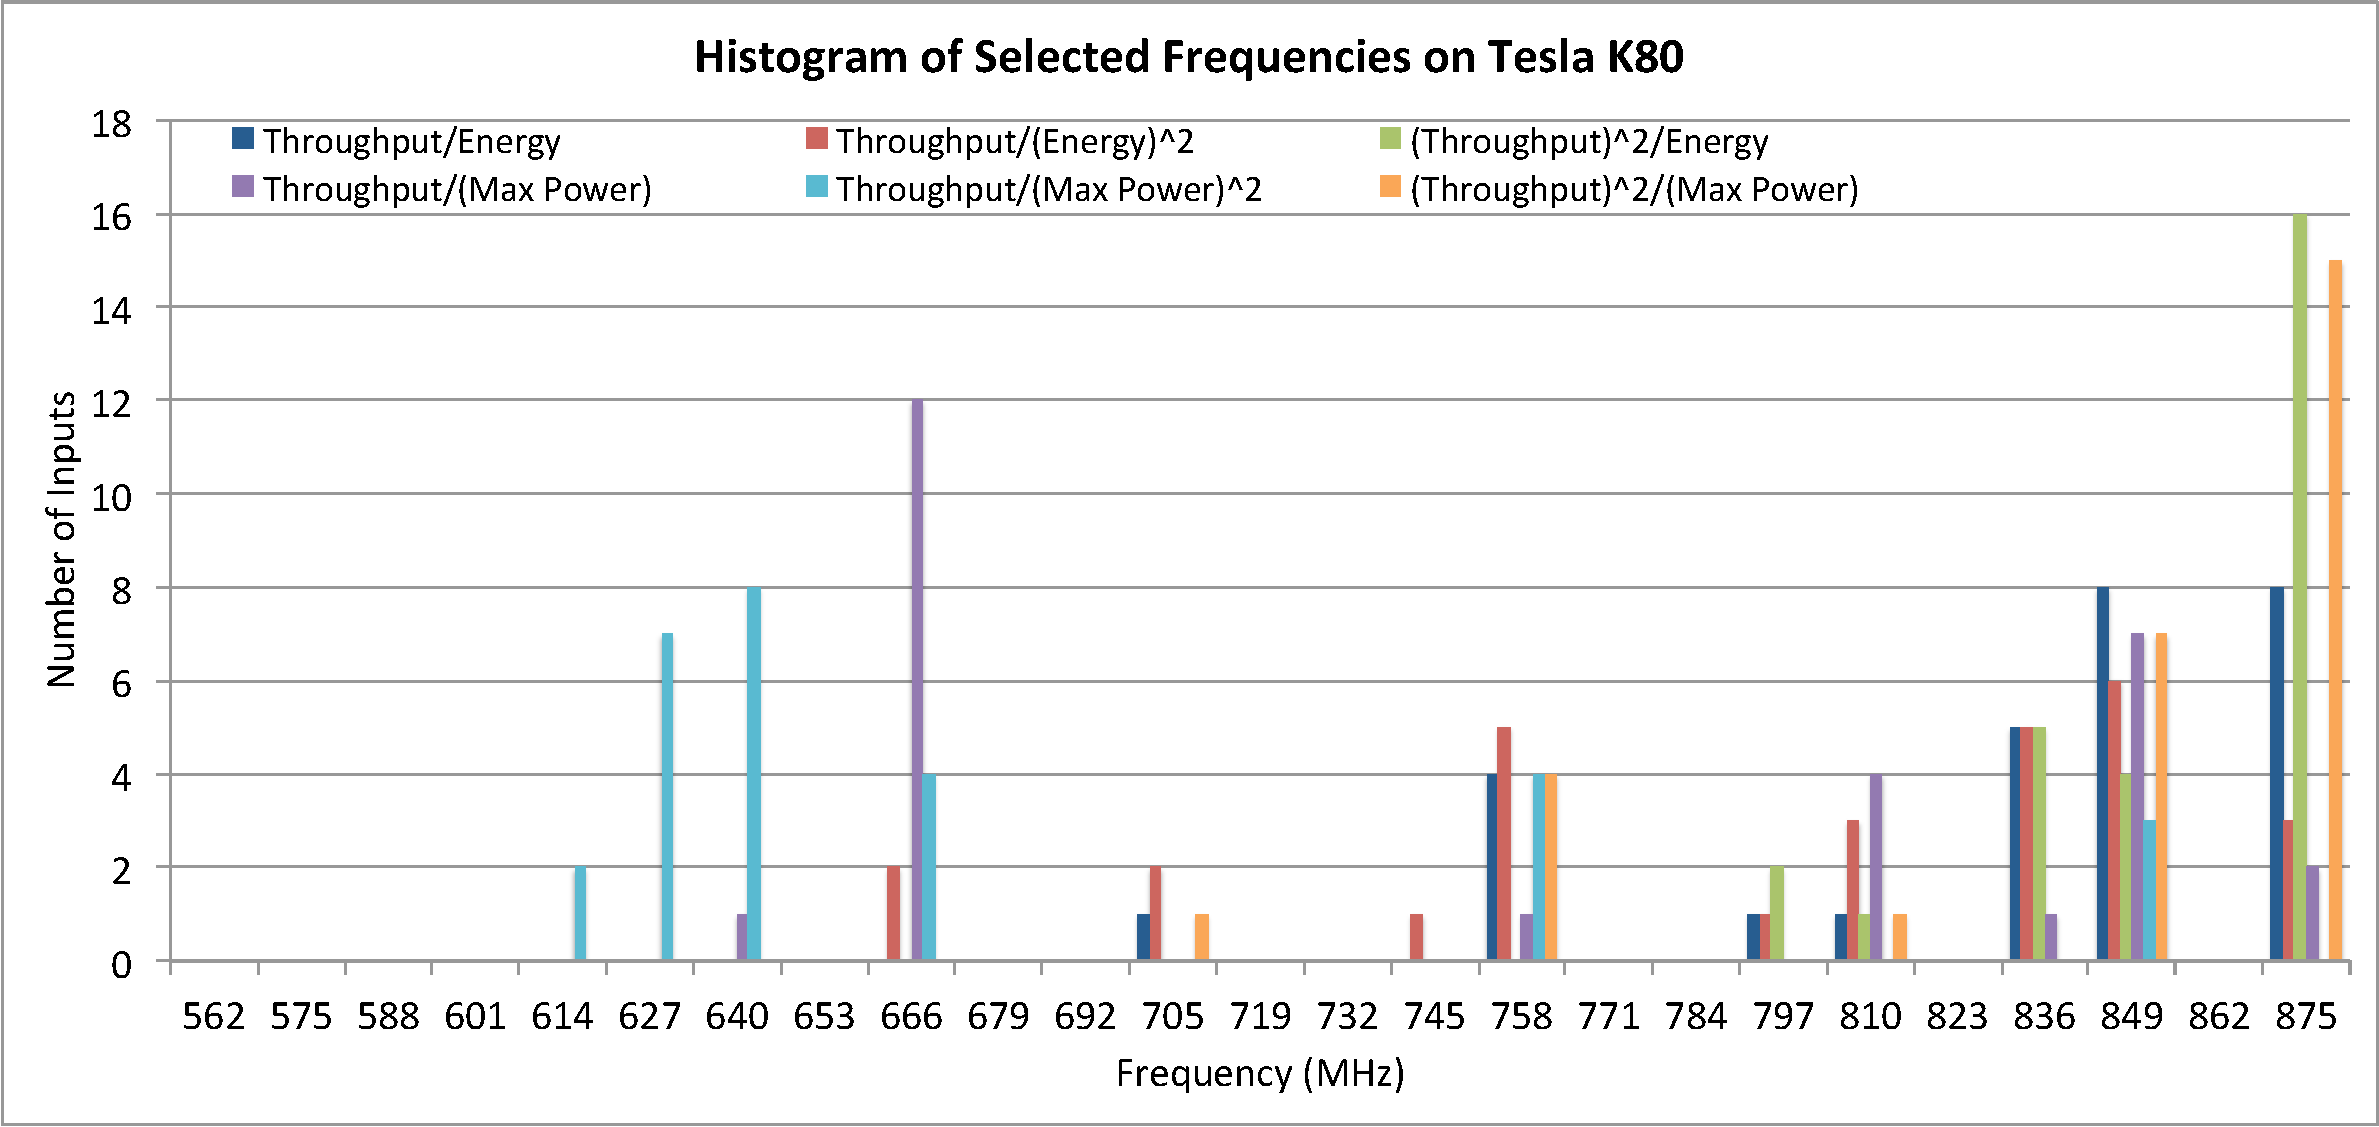
\includegraphics[scale=0.4]{figs/histo_k80.pdf}
   \caption{Frequencies selected on the Tesla K80 for various optimization objectives}
   \label{fig:histo-k80}
\end{figure*}

\subsection{Distributed Sort}

\begin{figure}
% Weak scaling type with 1GB per 
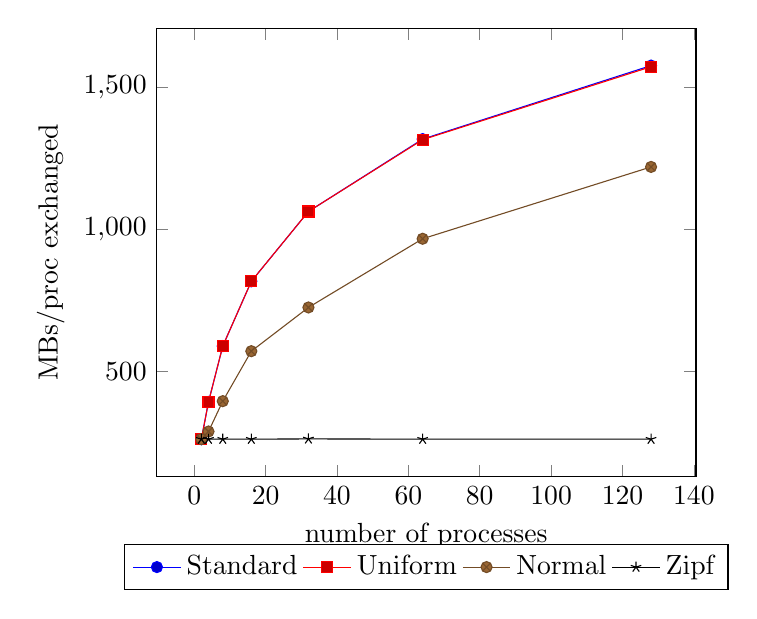
\begin{tikzpicture} 
\begin{axis}[ 
	xlabel={number of processes}, 
	ylabel={MBs/proc exchanged},
	legend style={at={(0.5,-0.15)}, 
	anchor=north,legend columns=-1}
	] 
  
  \addplot coordinates { 
    (2, 262) 
    (4, 393) 
    (8, 590) 
    (16, 818) 
    (32, 1064) 
    (64, 1319) 
    (128, 1578) 
  }; 
  
  \addplot coordinates { 
    (2, 262) 
    (4, 393) 
    (8, 590) 
    (16, 818) 
    (32, 1064) 
    (64, 1317) 
    (128, 1574) 
  }; 
  
  % gauss
%  \addplot coordinates { 
%    (2, 262) 
%    (4, 376) 
%    (8, 574) 
%    (16, 815) 
%    (32, 1048) 
%    (64, 1317) 
%    (128, 1579) 
%  }; 

  \addplot coordinates { 
    (2, 262) 
    (4, 289) 
    (8, 396) 
    (16, 572) 
    (32, 726) 
    (64, 968) 
    (128, 1221) 
  }; 
  
  % Zipf
%  \addplot coordinates { 
%    (2, 262) 
%    (4, 393) 
%    (8, 589) 
%    (16, 819) 
%    (32, 1064) 
%    (64, 1318) 
%    (128, 1576) 
%  }; 
  
  \addplot coordinates { 
    (2, 262) 
    (4, 262) 
    (8, 262) 
    (16, 262) 
    (32, 263) 
    (64, 262) 
    (128, 262) 
  }; 
  
  \legend{Standard,Uniform,Normal,Zipf} 

\end{axis} 
\end{tikzpicture}
\caption{\label{fig:comm} Communication costs of the distributed sorting algorithms in the style of weak scalability with a grain size of 1GB long integers per process. Standard refers to samplesort without any reassignment of ranks. The rest of the curves correspond to different data distributions with reassignment of ranks prior to data exchange. As expected, swapping of ranks makes almost no difference in case of uniform distributions, helps a little in case of a normal distribution and leads to almost fixed communication costs for skewed distributions like Zipf.}
\end{figure}
